\documentclass[11pt,twocolumn]{article}
\usepackage[margin=1in]{geometry}
\usepackage{amsmath,amssymb,amsfonts}
\usepackage{booktabs}
\usepackage{graphicx}
\usepackage{microtype}
\usepackage{hyperref}
\hypersetup{hidelinks}
\usepackage{subcaption}
\usepackage{enumitem}
\usepackage{amsthm}
\newtheorem{definition}{Definition}

\newcommand{\tva}{\textsf{TVA}}
\newcommand{\tvv}{\textsf{TVV}}
\newcommand{\valq}{\mathrm{Val}_{q}}
\newcommand{\taufill}{\tau_{\mathrm{fill}}}
\newcommand{\tauanchor}{\tau_{q}}

\title{Topological Void Validation:\\
       Density-Controlled and Role-Aware Evaluation\\
       of Predicted Research Voids}
\author{Kris Pan \\ Independent Researcher}
\date{}

\begin{document}

\twocolumn[
  \maketitle
  \begin{@twocolumnfalse}
  \begin{center}
  \begin{minipage}{0.92\textwidth}
  \textbf{Abstract.}
Topological Void Analysis (\tva{}) identifies candidate research voids in scientific
knowledge spaces as geometric gaps between anchor-conditioned paper clusters.
A natural validation question is whether future papers fill these predicted voids.
We show that raw fill rate---whether any future paper appears near a void's
midpoint---fails as a validation target for three compounding reasons.
First, it is confounded by local corpus density: a hot-zone baseline that samples
high-density anchor-adjacent pairs outperforms \tva{} on raw fill (36\% vs.\ 28\%),
but this apparent advantage disappears under a density-matched baseline
(25\%; \tva{}/B2 lift $= 1.12\times$, 95\% CI $\lbrack 0.85, 1.48\rbrack$, not significant).
Second, it is limited by anchor observability: only 5--7\% of future papers are
anchor-eligible per split, so many unfilled voids should be treated as right-censored
rather than invalid.
Third, even the geometric threshold itself is density-confounded: a fixed threshold of
0.82 corresponds to a 35.7\% average null occupancy rate, ranging from 1\% to 99\%
across anchor-density cells.
Under a null-calibrated threshold ($\taufill \approx 0.841$), fill rates collapse from
$\sim$27\% to $\sim$0.7\%, confirming that most raw fills are null-zone noise.
Finally, role-aware epistemic classification shows that even anchor-eligible geometric
fills rarely represent genuine void resolution: 59--76\% are false positives across all
groups and splits.
These findings motivate a three-layer validation framework---calibrated geometric
closure, anchor eligibility, and epistemic role---and establish that raw fill rate
measures future local activity near predicted voids but does not validate epistemic
closure.
  \end{minipage}
  \end{center}
  \vspace{1em}
  \end{@twocolumnfalse}
]

\section{Introduction}

Classical information retrieval asks: given a query, which existing documents are
relevant? Topological Void Analysis (\tva{}) asks: given an anchor concept, what
relevant knowledge is \emph{absent}?
\tva{} identifies candidate research voids as geometric gaps in an embedding-induced
knowledge space---regions between anchor-conditioned paper clusters where expected
connections, evidence, or conceptual bridges are missing.

Validating predicted voids requires asking: do they correspond to real epistemic gaps,
or to geometric artifacts? The natural operationalization is temporal fill rate:
does any future paper appear near the void's predicted midpoint?
This measure appears transparent, but we show it is confounded at every layer.

\textbf{Contributions:}
\begin{enumerate}
\item Raw temporal fill rate is strongly confounded by local historical density and
  research momentum.
\item A density-matched baseline shows that the apparent \tva{} disadvantage is not
  statistically significant (\tva{}/B2 lift $1.12\times$, CI $[0.85,1.48]$).
\item Fixed cosine thresholds are not portable: 0.82 has 35.7\% average null FPR;
  calibrated thresholds collapse raw fill to $\sim$0.7\%.
\item Anchor eligibility exposes an observability limit: only $\sim$6\% of future
  papers are anchor-eligible; unfilled voids are right-censored, not invalid.
\item Role-aware classification confirms that geometric fill substantially
  overestimates epistemic resolution (59--76\% FP across all groups).
\end{enumerate}

\textbf{Scope.} This paper concerns static retrospective validation against a
pre-committed future corpus window. Dynamic event-driven extensions are outside scope.

\section{Background}

\subsection{Topological Void Analysis}

\tva{} operates on a corpus embedded with BGE-M3 ($d=1024$, cosine similarity).
For anchor $q$ and source papers $A$, $B$, a candidate void satisfies four conditions:
(C1)~domain cohesion; (C2)~calibrated marginality; (C3)~sparse lexical bridge;
(C4)~midpoint vacancy. The midpoint is:
\[
m(A,B) = \frac{\mathbf{a}+\mathbf{b}}{\|\mathbf{a}+\mathbf{b}\|} \in \mathbb{S}^{1023}.
\]

\subsection{Temporal Validation in LBD}

Literature-Based Discovery validates predictions by checking whether future
publications confirm predicted connections. Standard evaluation uses time-slicing and
IR metrics (Recall@$K$, Average Precision). \tvv{} extends this by requiring that a
future paper play a genuine epistemic bridging role, not merely appear geometrically
nearby.

\subsection{Research Momentum and Dense-Region Confounding}

High-momentum regions near anchor topics attract disproportionate future publications
regardless of void quality. Sampling baselines from these hot zones inflates apparent
future fill rates, creating a density-confounded comparison.

\section{Experimental Setup}

\subsection{Corpus and Temporal Splits}

arXiv metadata (cs.OS/AR/PL/SE/DC/NI/CR/AI/LG), three rolling splits:

\begin{table}[h!]
\centering
\caption{Temporal splits.}
\begin{tabular}{lcccc}
\toprule
Split & $T$ & Val window & Train & Val \\
\midrule
t3 & 2014 & 2015--2019 & $\sim$29k & $\sim$101k \\
t4 & 2016 & 2017--2021 & $\sim$35k & $\sim$171k \\
t5 & 2018 & 2019--2023 & $\sim$51k & $\sim$193k \\
\bottomrule
\end{tabular}
\end{table}

\subsection{TVA Void Generation}

10 anchor concepts $\times$ top-30 MMR voids = 300 candidate voids per split.

\subsection{Baselines}

\textbf{B1 (hot-zone):} 20 random pairs from top-300 anchor C1 pool per anchor.
Biased toward high-density, high-momentum regions.

\textbf{B2 (density-matched):} For each \tva{} void, select the B1-style pair with
midpoint local density $\rho(m) = \frac{1}{k}\sum \mathrm{sim}(m, \mathrm{kNN}_i(m))$
($k=20$) closest to the \tva{} void's midpoint density.

\subsection{Three-Layer Fill Predicate}

Anchor-eligible val papers:
\[
\valq = \{P \in \mathrm{Val}_t : \mathrm{sim}(P,q) \ge \tauanchor\},
\quad \tauanchor = \max(Q_{80}^{\mathrm{val}},\, Q_{90}^{\mathrm{train}})
\]

Geometric filler candidate: $P_V^* = \arg\max_{P \in \valq} \mathrm{sim}(P, m_V)$

Geometric closure:
\[
G(V) = \mathbf{1}[\mathrm{sim}(P_V^*, m_V) \ge \taufill(q, \rho(V), t)]
\]

Validated epistemic fill:
\[
\mathrm{Fill}(V) = G(V) \wedge R(P_V^*, A, B, q)
\]
where $R=1$ iff $\mathrm{role} \in \{\mathrm{TRUE\text{-}FILL, PARTIAL\text{-}FILL}\}$.

\textbf{Calibrated threshold:}
\[
\taufill(q,\rho,t) = Q_{1-\alpha}\bigl(\{\max_{P\in\valq}\mathrm{sim}(P,m_0) :
m_0 \in \mathrm{Null}(q,\rho,t)\}\bigr), \quad \alpha=0.05
\]

\section{Results}

\subsection{Finding 1: Raw Fill Rate Is Density-Confounded}

\begin{table}[h!]
\centering
\caption{Raw fill rates under legacy $\tau=0.82$. CI from 1000 bootstrap resamples (t5).}
\begin{tabular}{lccccc}
\toprule
Split & \tva{} & B1 (hot) & B2 (density) & \tva{}/B2 lift & 95\% CI \\
\midrule
t3 & 31\% & 32\% & 30\% & $1.03\times$ & -- \\
t4 & 26\% & 32\% & 23\% & $1.12\times$ & -- \\
t5 & 27\% & 36\% & 24\% & $1.12\times$ & [0.85, 1.48] \\
\bottomrule
\end{tabular}
\end{table}

B1 consistently outperforms \tva{} by up to $1.30\times$. After density matching (B2),
\tva{} achieves $1.03$--$1.12\times$ lift, but the t5 CI includes 1.0---not significant.

\subsubsection{Fixed Thresholds Are Not Portable}

\begin{table}[h!]
\centering
\caption{Calibrated threshold and null FPR@0.82 by density bucket (t5 mean).}
\begin{tabular}{lccc}
\toprule
Density bucket & Null p50 & $\taufill$ (p95) & FPR@0.82 \\
\midrule
Low  & 0.787--0.811 & 0.790--0.859 & 1--18\% \\
Mid  & 0.802--0.832 & 0.818--0.861 & 5--80\% \\
High & 0.810--0.854 & 0.841--0.881 & 28--99\% \\
Global mean & -- & \textbf{0.841} & \textbf{35.7\%} \\
\bottomrule
\end{tabular}
\end{table}

Under calibrated $\taufill$, fill rates collapse:
\tva{}: 27.3\%$\rightarrow$\textbf{0.7\%};\quad
B2: 24.3\%$\rightarrow$\textbf{0.7\%};\quad lift: $1.00\times$.

The $0.7\% < 5\%$ result is correct: \tva{} C1--C4 conditions select sparser bridge
regions than random density-matched pairs, so fewer reach the calibrated threshold.
Most raw fills at $\tau=0.82$ are null-zone occupancy, not significant geometric closure.

\begin{figure}[h!]
\centering
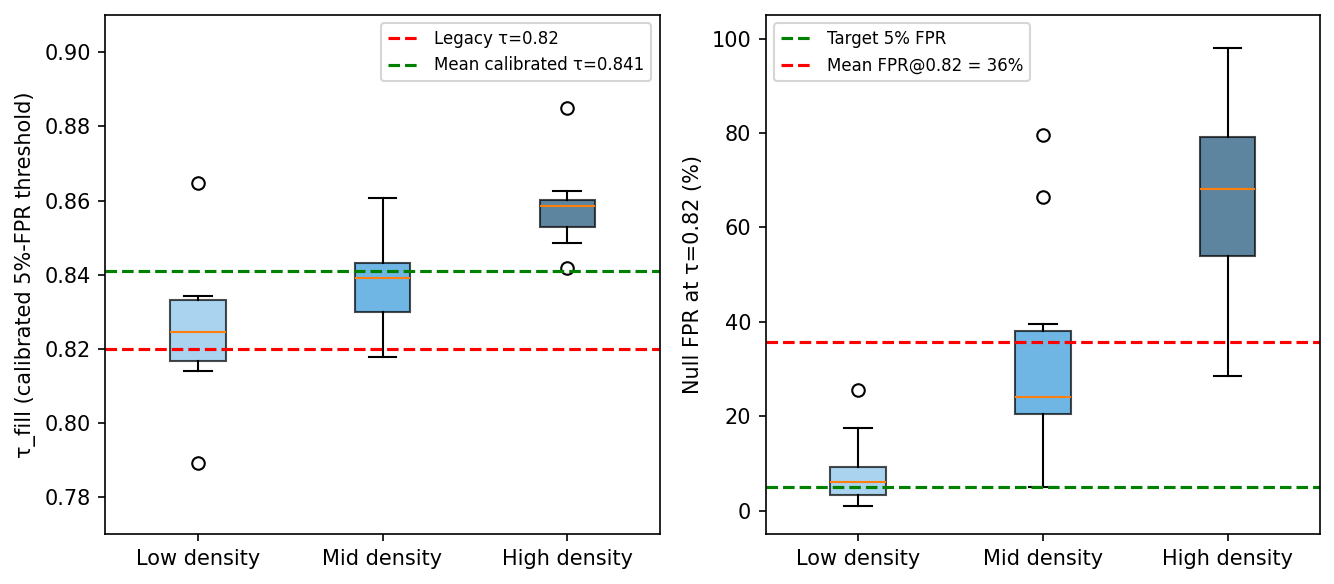
\includegraphics[width=0.95\textwidth]{figures/fig2_threshold_calibration.png}
\caption{Calibrated threshold by density bucket (left) and null FPR at 0.82 (right).
The fixed threshold 0.82 has 35.7\% average null FPR, reaching 99\% in high-density
anchor cells. Calibrated $\taufill\approx 0.841$ is stable across all splits.}
\end{figure}

\subsection{Finding 2: Anchor Eligibility Reveals Observability Limits}

\begin{table}[h!]
\centering
\caption{Anchor exposure (t5 sample). Mean sim and hybrid gate pass rate.}
\begin{tabular}{lcccc}
\toprule
Anchor & Mean sim & $\tauanchor$ & Pass rate & \tva{} fill \\
\midrule
sched\_opt & 0.520 & 0.582 & 5.8\% & 40\% \\
ebpf\_obs  & 0.495 & 0.547 & 6.5\% & 0\%  \\
virt\_hyp  & 0.498 & 0.555 & 7.7\% & 57\% \\
\textbf{Mean} & \textbf{0.503} & \textbf{0.563} & \textbf{6.2\%} & -- \\
\bottomrule
\end{tabular}
\end{table}

Only 5--8\% of val papers are anchor-eligible per split. Voids with pass rate $<10\%$
are flagged as \emph{underexposed}: their unfill status reflects observability limits,
not void invalidity. ebpf\_obs (6.5\% pass, 0\% fill) illustrates that non-zero
exposure does not guarantee eligible papers overlap predicted void neighborhoods.

\begin{figure}[h!]
\centering
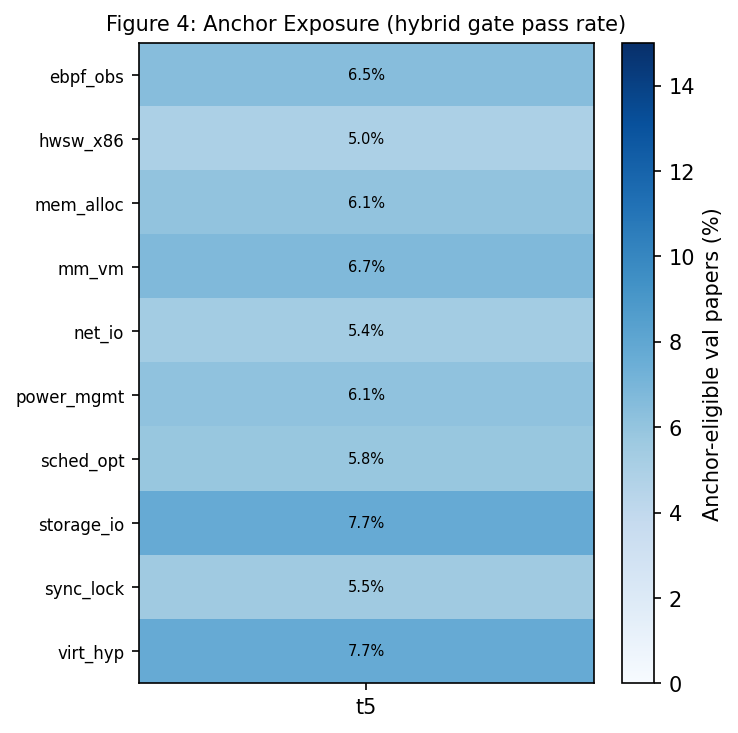
\includegraphics[width=0.55\textwidth]{figures/fig4_anchor_exposure.png}
\caption{Anchor eligibility pass rate (\%) by anchor and split (hybrid gate).
Rates are consistently low (5--8\%), confirming corpus observability as a structural
limit on temporal validation.}
\end{figure}

\subsection{Finding 3: Geometric Fill Rarely Equals Epistemic Fill}

\begin{table}[h!]
\centering
\caption{Epistemic role decomposition (t3/t4/t5 combined, 500 sampled cases).
Void res.\ = TRUE-FILL + PARTIAL-FILL; Boundary = IE + SE + SN; FP = FALSE-POSITIVE.}
\begin{tabular}{lccccc}
\toprule
Source & $n$ & Void res. & Boundary & FP & Score $\bar{s}$ \\
\midrule
TVA (gated)  & 98  & 0\% & 33\% & 69\% & 0.068 \\
B1 (gated)   & 73  & 0\% & 33\% & 70\% & 0.062 \\
B2 density   & 107 & 3\% & 36\% & 62\% & 0.104 \\
Near-miss    & 219 & 2\% & 13\% & 84\% & 0.043 \\
\bottomrule
\end{tabular}
\end{table}

59--76\% of gated raw fills are false positives across all groups and splits.
Near-miss controls show the highest FP rate (84\%) and lowest score, confirming that
geometric proximity carries some signal but is insufficient.
TVA and B1 are statistically indistinguishable; B2 performs marginally better.

\begin{figure}[h!]
\centering
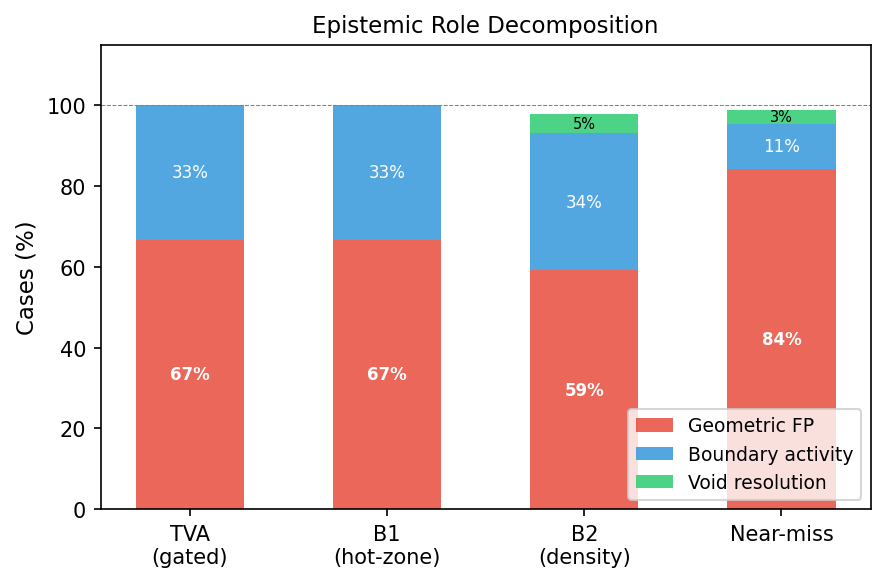
\includegraphics[width=0.75\textwidth]{figures/fig1_role_decomposition.png}
\caption{Epistemic role decomposition by source group (t5, 200 sampled cases).
Most raw fills are geometric false positives regardless of method. Near-miss
controls show the highest FP rate, confirming that geometric proximity is
a weak but non-zero signal.}
\end{figure}

\subsection{Case Studies}

Three representative cases from t4/t5:

\textbf{Case 1 -- Partial Fill} (arXiv:1912.06243, 2019, 18 citations):
Vehicular cloud multi-task offloading. $\mathrm{sim}(P,m)=0.835$. Contains 10+
task-offloading refs (B-side) but only 1 marginal virtualization ref (A-side).
Role: PARTIAL-FILL---one-sided bridging.

\textbf{Case 2 -- Boundary Expansion} (arXiv:2106.01441, 2021, 7 citations):
AI planning for heterogeneous system optimization. $\mathrm{sim}(P,m)=0.855$.
Zero kernel-scheduler refs; all 44 refs in heterogeneous HPC.
Role: INCREMENTAL-EXTENSION---pure boundary expansion along B-direction.

\textbf{Case 3 -- False Positive} (arXiv:1710.11590, 2017, 6 citations):
Energy-aware virtual network embedding. $\mathrm{sim}(P,m)=0.875$ (highest).
Zero storage I/O or NVMe refs. Anchor is storage I/O---completely unrelated.
Role: FALSE-POSITIVE---dense-region artifact.

\begin{figure}[h!]
\centering
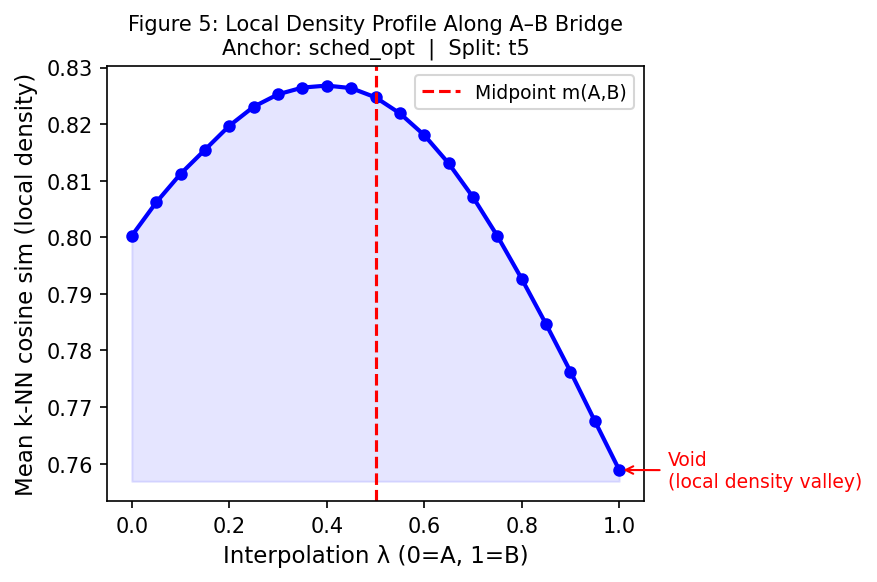
\includegraphics[width=0.75\textwidth]{figures/fig5_void_valley.png}
\caption{Local density profile along the A--B bridge for the highest-MMR void
in anchor sched\_opt (t5). The density valley at $\lambda\approx 0.5$ marks
the void midpoint region---two dense source communities with a less-occupied bridge.}
\end{figure}

\section{Discussion}

\subsection{Raw Fill Fails for Three Reasons}

Raw fill conflates void quality with sociotechnical realization rate:
(1)~hot-zone baselines are biased by local momentum;
(2)~fixed thresholds are not portable across anchor-density regimes;
(3)~anchor-eligible future papers are sparse ($\sim$6\%), right-censoring many unfilled voids.

\subsection{From Geometric Occupancy to Role Decomposition}

Future papers near void midpoints decompose into true fills, boundary expansions, and
false positives. The scarcity of true fills reveals that genuine epistemic closure is
a much stricter condition than geometric occupancy.
\emph{Geometric closure and anchor eligibility are screening conditions; epistemic
role is the validation condition.}

\subsection{Descriptive, Not Evaluative}

\tvv{} classifies the type of validation evidence produced by future literature, not
the intrinsic merit of papers. Boundary expansion and incremental extension are
valuable scientific activities.

\subsection{Dynamic Extension (Future Work)}

These results suggest a natural extension: instead of asking whether a predicted void
is eventually filled within a fixed window, one can classify each newly arriving paper
by its pre-insertion topological impact on the existing knowledge space.
This dynamic formulation is outside the scope of the present work.

\subsection{Threats to Validity}

(1)~\emph{Embedding dependence}: all metrics use BGE-M3.
(2)~\emph{Threshold sensitivity}: calibration uses 200 null midpoints per cell.
(3)~\emph{Corpus coverage}: fills outside arXiv are unobservable; unfilled voids are right-censored.
(4)~\emph{LLM classification}: single model, no inter-rater reliability.
(5)~\emph{Domain specificity}: CS arXiv categories only.

\section{Related Work}

\textbf{Literature-Based Discovery.}
Swanson's ABC model and subsequent LBD work validate predictions by checking future
publication appearance. \tvv{} extends this tradition by requiring epistemic bridging
role, not merely geometric proximity.

\textbf{Novelty and First-Story Detection.}
Topic Detection and Tracking introduced first-story detection; novelty detection in IR
measures whether a document adds new information relative to a query set. Our
first-filler intuition shares the event-ordering structure but operates on knowledge
structure rather than event reporting.

\textbf{Structural Holes and Scientometrics.}
Burt's structural hole theory shows brokers spanning gaps accumulate informational
advantage. Our density-matched baseline directly controls for hot-zone momentum.

\textbf{Dense-Region Bias in Embeddings.}
Anisotropy in high-dimensional text embeddings compresses cosine similarities into a
narrow range. We show this anisotropy makes fixed thresholds non-portable in
downstream void validation.

\textbf{Scientific Claim Verification.}
Epistemic classification of scientific contributions---argumentative zoning,
overclaiming detection---provides precedents for our role-aware rubric.

\section{Conclusion}

Temporal validation of predicted research voids requires separating geometric occupancy,
density bias, anchor observability, and epistemic role.
Under density matching, \tva{}'s apparent disadvantage disappears but is not
statistically significant. Under null-calibrated thresholds, fill rates collapse to
$\sim$0.7\%---most raw fills were null-zone noise.
Role-aware classification confirms that genuine epistemic bridging is rare even among
geometrically close, anchor-eligible future papers.

We propose a three-layer validation framework and leave two open questions for future
work: (1)~scalable role-aware validation without prohibitive LLM cost;
(2)~dynamic event-driven extensions in which each arriving paper updates knowledge-space
state.

\bigskip
\noindent\textbf{Acknowledgements.} TODO.

\bibliographystyle{plain}
\bibliography{paper2}

\end{document}
